\begin{appendices}

\chapter{Fichiers LQL Nagios}
\label{chapterAnnexe:fichiersLQLNagios}

Cette annexe permet une vue sur les fichiers LQL permettant la r\'ecup\'eration des informations de Nagios. 
Ces informations sont ensuite trait\'ees par le service Web qui se charge de remplir ou actualiser la base de donn\'ees en cons\'equence.

\subsubsection{R\'ecup\'eration des salles}

La requ\^ete~\ref{annexe:nagiosGetHostGroups} permet d'interroger Nagios afin de r\'ecup\'erer les salles qu'il surveille.
Ces salles sont appel\'ees \textit{hostgroups} et contiennent des machines appel\'ees \textit{hosts}.
Parmi ces \textit{hostgroups}, les imprimantes, serveurs et autres ressources sont exclues pour ne retenir que les salles.
La socket Nagios retournera alors le nom de la salle, le nombre de machines qu'elle contient, et la liste des machines qui font partie du groupe.

\vspace{0.20cm}

\begin{figure}[!ht]
	\lstinputlisting[language=LQL]{codes/nagiosGetHostGroups.ngs}
	\caption{Code LQL de r\'ecup\'eration des salles que surveille Nagios}
	\label{annexe:nagiosGetHostGroups}

\end{figure}

\subsubsection{R\'ecup\'eration des machines}

La requ\^ete~\ref{annexe:nagiosGetResources} permet d'interroger Nagios afin de r\'ecup\'erer toutes les machines qui peuvent poss\'eder un utilisateur de connect\'e.
En fait, il est demand\'e la r\'ecup\'eration de tous les services ayant acc\`es \`a l'information \textsf{check\_whoisloggedin}.
Cette information permet de r\'ecup\'erer l'identifiant de la personne connect\'e \`a une machine, si tant est qu'une personne y est connect\'ee.
Il y a pour chaque machine, un service portant ce nom, cela revient donc \`a demander tous les ordinateurs.
La socket Nagios retournera alors le nom de la machine, son adresse IP, le \textsf{host\_groups} donc le nom de la salle \`a laquelle elle appartient, son \'etat et enfin l'utilisateur connect\'e s'il y en a un.

\begin{figure}[!ht]
	\lstinputlisting[language=LQL]{codes/nagiosGetResources.ngs}
	\caption{Code LQL de r\'ecup\'eration des machines que surveille Nagios}
	\label{annexe:nagiosGetResources}

\end{figure}

\subsubsection{R\'ecup\'eration de tous les utilisateurs connect\'es}

La requ\^ete~\ref{annexe:nagiosGetUsersLogged} permet d'interroger Nagios afin de r\'ecup\'erer seulement la liste des utilisateurs connect\'es sur les machines sous surveillance.
Il est demand\'e la r\'ecup\'eration de tous les services parmi lesquels il n'est gard\'e que ceux sur lesquels un utilisateur peut se connecter.
De plus, les messages de Nagios concernant un \'eventuel probl\`eme dans la r\'ecup\'eration de l'information sont \'ecart\'es.
Seul les utilisateurs \og corrects\fg{} sont gard\'es.

\vspace{0.20cm}

\begin{figure}[!ht]
	\lstinputlisting[language=LQL]{codes/nagiosGetUsersLogged.ngs}
	\caption{Code LQL de r\'ecup\'eration des utilisateurs connect\'es sur les machines que surveille Nagios}
	\label{annexe:nagiosGetUsersLogged}

\end{figure}

\chapter{Retours de requ\^ete LQL}
\label{chapterAnnexe:reponseLQLNagios}

Cette annexe permet une vue sur les informations qui sont retourn\'ees par une requ\^ete LQL.
Les informations se pr\'esentent toujours sous la m\^eme forme : une ligne qui est compos\'ee des diff\'erentes colonnes demand\'ees dans la requ\^ete.
Les colonnes sont s\'epar\'ees par un \textsf{";" (point-virgule)}.

\subsubsection{Retour lors d'une r\'ecup\'eration des salles}

La r\'eponse~\ref{annexe:reponseNagiosGetHostGroups} correspond \`a l'ex\'ecution de la requ\^ete~\ref{annexe:nagiosGetHostGroups} sur le serveur contenant Nagios.

\begin{figure}[!ht]
	\centering
	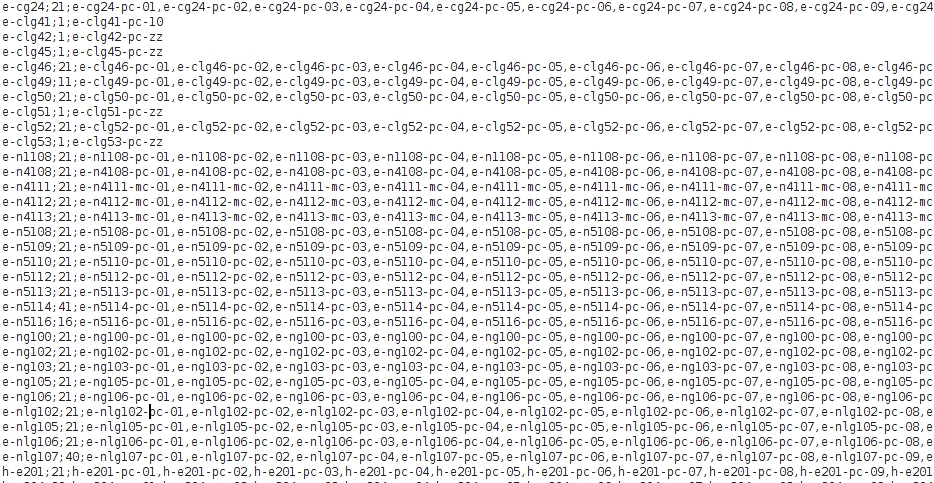
\includegraphics[scale=0.45]{reponseNagiosGetHostGroups.jpg}
	\caption{R\'eponse lors d'une requ\^ete de r\'ecup\'eration de salle}
	\label{annexe:reponseNagiosGetHostGroups}

\end{figure}

\subsubsection{Retour lors d'une r\'ecup\'eration des machines}

La r\'eponse~\ref{annexe:reponseNagiosGetResources} correspond \`a l'ex\'ecution de la requ\^ete~\ref{annexe:nagiosGetResources} sur le serveur contenant Nagios.

\begin{figure}[!ht]
	\centering
	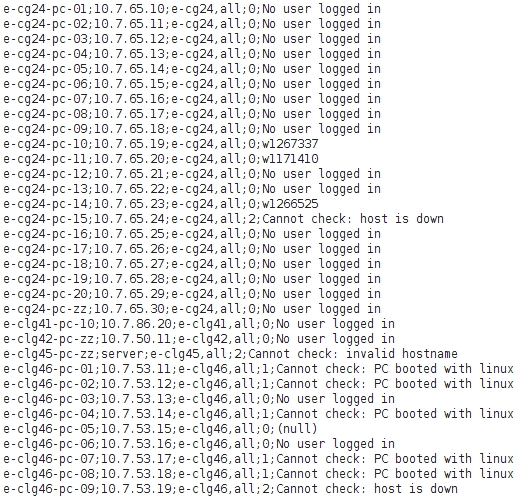
\includegraphics[scale=0.5]{reponseNagiosGetResources.jpg}
	\caption{R\'eponse lors d'une requ\^ete de r\'ecup\'eration des machines}
	\label{annexe:reponseNagiosGetResources}

\end{figure}

\subsubsection{Retour lors d'une r\'ecup\'eration des utilisateurs}

La r\'eponse~\ref{annexe:reponseNagiosGetUsersLogged} correspond \`a l'ex\'ecution de la requ\^ete~\ref{annexe:nagiosGetUsersLogged} sur le serveur contenant Nagios.

\begin{figure}[!ht]
	\centering
	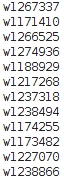
\includegraphics[scale=0.5]{reponseNagiosGetUsersLogged.jpg}
	\caption{R\'eponse lors d'une requ\^ete de r\'ecup\'eration des utilisateurs}
	\label{annexe:reponseNagiosGetUsersLogged}

\end{figure}

\chapter{Base de donn\'ees}
\label{chapterAnnexe:baseDeDonnees}

Cette annexe permet d'avoir une vue sur les relations entre tables ainsi que sur leur contenu.
Dans un premier temps, une description rapide des tables sera faite.
Ensuite, le diagramme de leur agencement les unes avec les autres sera donn\'e en entier.
Enfin, ce diagramme sera d\'ecoup\'e en diff\'erentes parties pour plus de visibilit\'e.

\subsubsection{Description des tables}

\noindent {\YuukouII} est compos\'e de 14 tables :

\begin{itemize}
	\item[\textbf{\textsf{yuukou\_rooms}}] contient les descriptions des salles informatiques;
	\item[\textbf{\textsf{yuukou\_resources}}] contient les descriptions des ordinateurs appartenant \`a une salle particuli\`ere;
	\item[\textbf{\textsf{yuukou\_users}}] contient les descriptions des utilisateurs;
	\item[\textbf{\textsf{yuukou\_last}}] contient les historiques de toutes les connexions pass\'ees sur les ordinateurs;
	\item[\textbf{\textsf{yuukou\_who}}] contient les historiques de toutes les connexions en cours sur les ordinateurs;
	\item[\textbf{\textsf{yuukou\_mapping\_location}}] contient les informations sur les diff\'erents campus de l'Universit\'e, le but \'etant de faire un lien avec la localisation de la table \textsf{yuukou\_rooms} et la description compl\`ete de cette localisation contenue dans la table de \textit{mapping};
	\item[\textbf{\textsf{yuukou\_mapping\_room}}] contient les diff\'erentes correspondances entre le nom des salles telles qu'elles sont appel\'ees dans {\YuukouII} et le nom des salles r\'ecup\'er\'ees avec les emplois du temps;
	\item[\textbf{\textsf{yuukou\_timetables}}] contient les diff\'erentes informations concernant un \'el\'ement de l'emploi du temps;
	\item[\textbf{\textsf{yuukou\_settings}}] contient les diff\'erentes informations de configuration de \YuukouII;
	\item[\textbf{\textsf{yuukou\_groups}}] contient les descriptions des groupes de logiciels;
	\item[\textbf{\textsf{yuukou\_software}}] contient les descriptions des logiciels;
	\item[\textbf{\textsf{yuukou\_groups\_software}}] contient les diff\'erents liens entre un groupe de logiciels et tous les logiciels les composant;
	\item[\textbf{\textsf{yuukou\_rooms\_groups}}] contient les diff\'erents liens entre les salles et tous les groupes de logiciels les composant;
	\item[\textbf{\textsf{yuukou\_roms\_software}}] contient les diff\'erents liens entre les salles et tous les logiciels, n'appartenant pas \`a un groupe de logiciels, les composant.
	
\end{itemize}


\subsubsection{Structure g\'en\'erale}

La figure~\ref{annexe:modeleGeneral} pr\'esente la structure g\'en\'erale du projet \YuukouII.
Elle s'articule en diff\'erentes sous-parties : la partie archivage, logicielle, emploi du temps, mapping et configuration.

\begin{figure}[!ht]
	\centering
	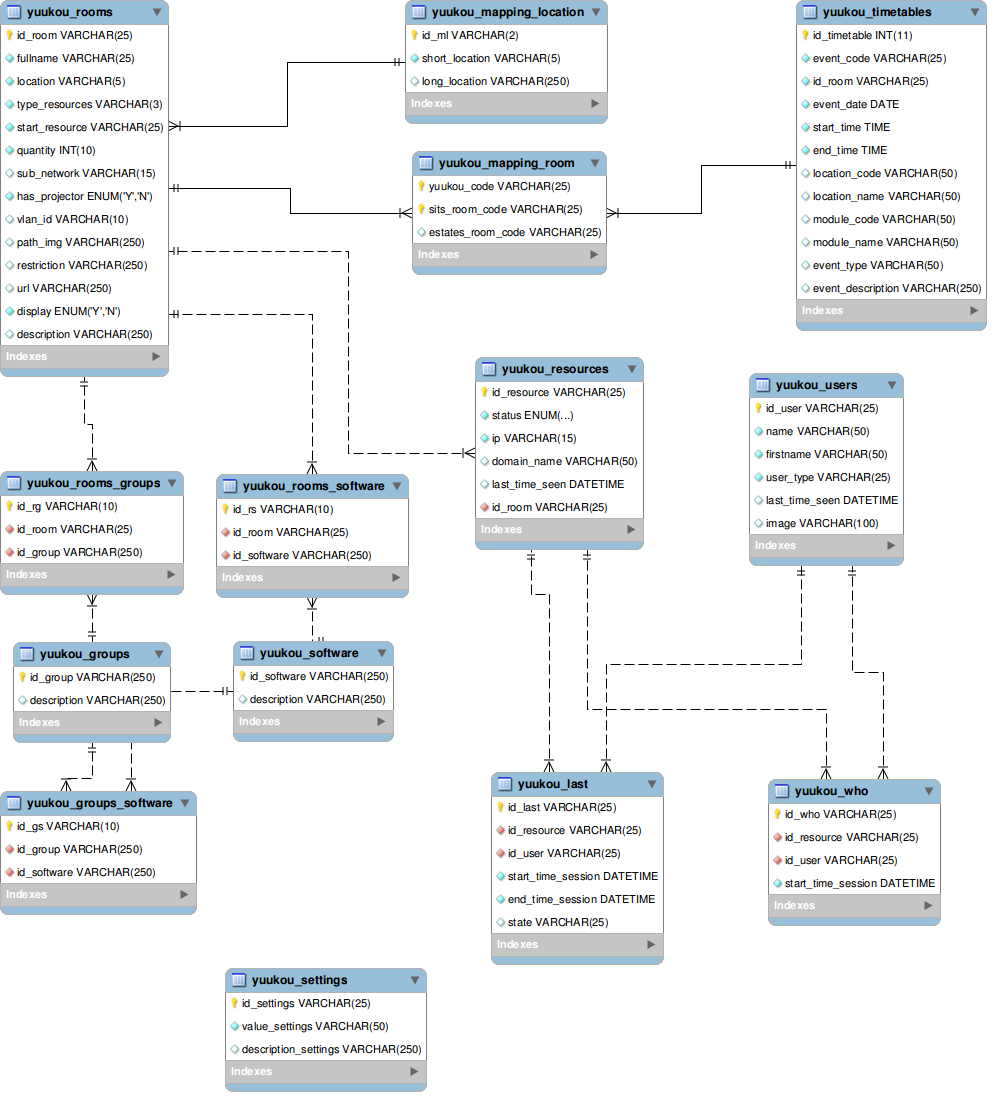
\includegraphics[scale=0.40]{modeleGeneral.png}
	\caption{Structure g\'en\'erale de la base de donn\'ees}
	\label{annexe:modeleGeneral}

\end{figure}

\clearpage

\subsubsection{Partie archivage}

La partie archivage a pour r\^ole le stockage des donn\'ees concernant d'une part l'historique des connexions actuelles et d'autre part, l'historique des connexions pass\'ees.

\begin{figure}[!ht]
	\centering
	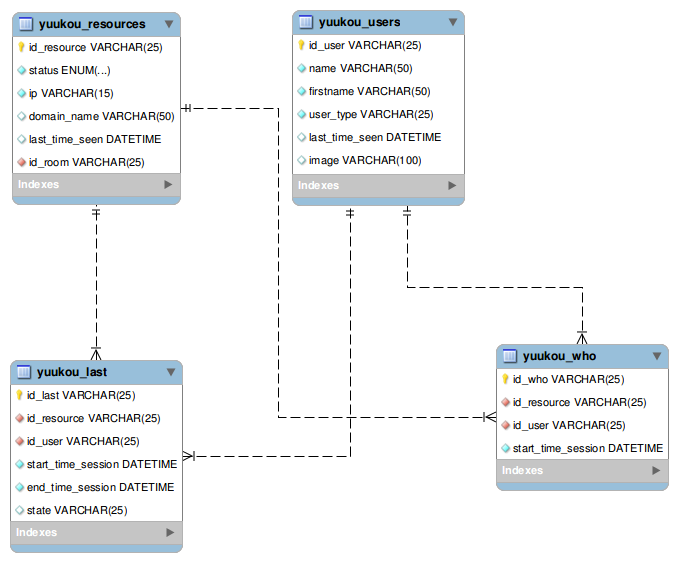
\includegraphics[scale=0.35]{modeleArchivage.png}
	\caption{Structure de la partie archivage de la base de donn\'ees}
	\label{annexe:modeleArchivage}

\end{figure}


\subsubsection{Partie logicielle}

La partie logicielle a pour r\^ole de lier les informations de configuration logicielle avec les salles informatiques de l'Universit\'e.

\clearpage

\begin{figure}[!ht]
	\centering
	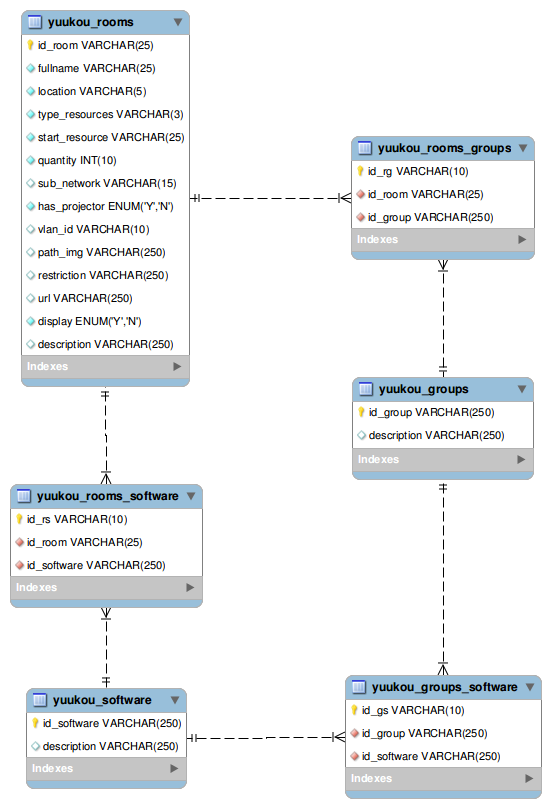
\includegraphics[scale=0.35]{modeleLogiciel.png}
	\caption{Structure de la partie logicielle de la base de donn\'ees}
	\label{annexe:modeleLogiciel}

\end{figure}


\subsubsection{Partie emploi du temps}

La partie emploi du temps a pour r\^ole de lier les informations d'emploi du temps \`a une salle en passant par une table de mapping faisant le lien entre le nom d'une salle dans {\YuukouII} et le nom d'une salle utilis\'e par les services centraux informatiques lors de la g\'en\'eration des emplois du temps.

\clearpage

\begin{figure}[!ht]
	\centering
	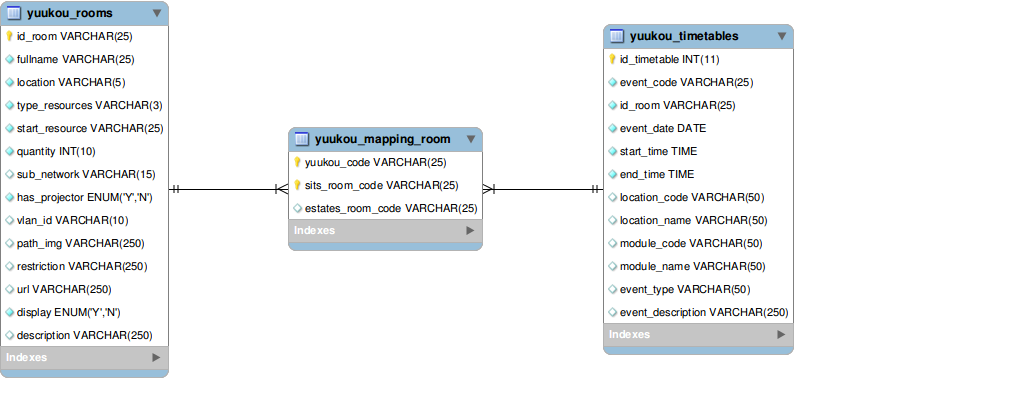
\includegraphics[scale=0.35]{modeleEmploiDuTemps.png}
	\caption{Structure de la partie emploi du temps de la base de donn\'ees}
	\label{annexe:modeleEmploiDuTemps}

\end{figure}

\subsubsection{Partie \textit{mapping} avec les salles}

La partie \textit{mapping} avec les salles a pour r\^ole de faire le lien entre la localisation d'une salle et les informations concernant cette localisation.

\begin{figure}[!ht]
	\centering
	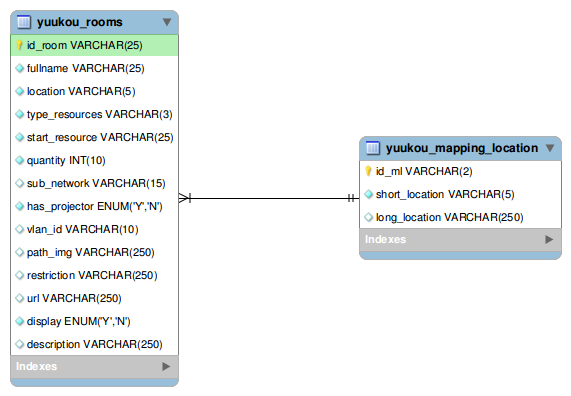
\includegraphics[scale=0.35]{modeleMapping.png}
	\caption{Structure de la partie \textit{mapping} de la base de donn\'ees}
	\label{annexemodeleMapping}

\end{figure}

\subsubsection{Partie configuration}

La partie configuration a pour r\^ole de stocker tous les param\`etres permettant de g\'erer un cycle du service Web pendant son ex\'ecution.

\begin{figure}[!ht]
	\centering
	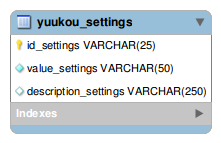
\includegraphics[scale=0.35]{modeleConfiguration.png}
	\caption{Structure de la partie configuration de la base de donn\'ees}
	\label{annexe:modeleConfiguration}

\end{figure}

\chapter{Exemples de retours JSON}
\label{chapterAnnexe:exempleJSON}

Cette annexe permet d'avoir une vue sur des exemples de retours corrects lors d'appels de fonctions du service Web.
Deux retours de m\'ethodes sont propos\'es ici.

Le code JSON~\ref{annexe:getsitesinformation} correspond au retour de l'appel \`a la fonction \textbf{getSitesInformation ()} du service Web.

\begin{figure}[!ht]
	\centering
	\lstinputlisting[language=JSON]{codes/getSitesInformation.json}
	\caption{Exemple de retour de la fonction \textbf{getSitesInformation ()}}
	\label{annexe:getsitesinformation}

\end{figure}

\clearpage

Le code JSON~\ref{annexe:getlistrooms} correspond au retour de l'appel \`a la fonction \textbf{getListRooms ()} du service Web.

\begin{figure}[!ht]
	\centering
	\lstinputlisting[language=JSON]{codes/getListRooms.json}
	\caption{Exemple de retour de  la fonction \textbf{getListRooms ()}}
	\label{annexe:getlistrooms}

\end{figure}

\end{appendices}

\clearpage
